\documentclass[a4paper]{report}
\usepackage[margin=1.9in]{geometry}

\usepackage[utf8]{inputenc}
\usepackage[T1]{fontenc}
\usepackage{textcomp}
\usepackage[spanish]{babel}
\decimalpoint

\usepackage{csquotes}
\usepackage[sorting=none]{biblatex}
\addbibresource{refs.biblatex}

\usepackage{amsmath, amssymb}
\usepackage{amsthm}
\usepackage{bm}
\usepackage{braket}

\usepackage{graphicx}

\usepackage{hyperref}
\hypersetup{
    colorlinks,
    citecolor=red,
    filecolor=black,
    linkcolor=blue,
    urlcolor=black
}

\usepackage[marginal]{showlabels}

\DeclareMathOperator{\R}{\mathbb{R}}
\DeclareMathOperator{\C}{\mathbb{C}}
\DeclareMathOperator{\N}{\mathbb{N}}
\DeclareMathOperator{\Z}{\mathbb{Z}}
\DeclareMathOperator{\F}{\mathbb{F}}

\let\H\relax
\DeclareMathOperator{\H}{\mathcal H}
\DeclareMathOperator{\Sz}{\mathcal S}

\DeclareMathOperator{\dom}{Dom}
\DeclareMathOperator{\prob}{Prob}
\DeclareMathOperator{\id}{id}
\DeclareMathOperator{\Tr}{Tr}
\DeclareMathOperator{\tr}{tr}
\DeclareMathOperator{\Op}{Op}
\DeclareMathOperator{\W}{W}
\DeclareMathOperator{\Fr}{\mathcal{F}\!}

\newtheorem{definition}{Definición}
\newtheorem{theorem}{Teorema}
\newtheorem{proposition}{Proposición}
\newtheorem{lemma}{Lema}
\newtheorem{corollary}{Corolario}
\newtheorem{example}{Ejemplo}
\newtheorem{axiom}{Postulado}
\newtheorem{remark}{Observación}

\hfuzz=50pt

\title{Funciones de Wigner en el Espacio de Fase Discreto}
\author{Ernesto Camacho Ramírez}

\begin{document}
  \maketitle

  \tableofcontents

  \section{Introducción}

  El número de elementos de un conjunto general de
  operadores cuánticos unitarios sobre estados de $n$-qudit
  generalmente crece exponencialmente con $n$. Una excepción
  importante a ésta regla involucra el conjunto de
  operadores de Clifford que actúan sobre estados
  estabilizadores. Éstos estados juegan un papel importante
  en la corrección de errores cuánticos
  \cite{gottesmanHeisenbergRepresentationQuantum1998} y son
  cerrados bajo la acción de las compuertas de Clifford. La
  simulación eficiente de dichos sistemas con una
  computadora clásica se demostró con el algoritmo tableau
  de Aaronson y Gottesman \cite{
    aaronsonImprovedSimulationStabilizer2004,
  gottesmanHeisenbergRepresentationQuantum1998} para qubits
  ($d=2$). La busqueda de un explicación de por qué un
  algoritmo tan eficiente es posible para la simulación de
  circuitos de Clifford ha sido un objeto de mucho estudio
  \cite{gottesmanFaultTolerantQuantumComputation1999,
    howardContextualitySuppliesMagic2014,
  mariPositiveWignerFunctions2012}. El progreso reciente ha
  sido resultado del trabajo de Wooters
  \cite{woottersWignerFunctionFormulationFiniteState1987},
  Eisert \cite{mariPositiveWignerFunctions2012}, Gross
  \cite{grossHudsonTheoremFinitedimensional2006} y Emerson
  \cite{howardContextualitySuppliesMagic2014}, quienes han
  formulado una nueva perspectiva basada en los espacios de
  fase discretos de estados y operadores en espacios de
  Hilbert finitos, utilizando funciones discretas de Wigner.
  Se ha demostrado que los estados estabilizadores tienen
  funciones de Wigner discretas definidas positivas y que
  los operadores de Clifford son mapeos definidos positivos.
  Esto implica que los circuitos de Clifford son simulables
  eficientemente en computadores clásicas. En sistemas de
  dimensiones impares, se ha demostrado que los estados
  estabilizadores son análogos discretos a los estados
  gaussianos en sistemas continuos
  \cite{grossHudsonTheoremFinitedimensional2006} y se ha
  demostrado que las compuertas del grupo de Clifford tienen
  Hamiltonianos armónicos subyacentes que conservan los
  puntos discretos del espacio de fase
  \cite{kociaSemiclassicalFormulationGottesmanKnill2017}.
  Esto significa que los circuitos de Clifford se pueden
  expresar mediante integrales de trayectoria truncadas en
  el orden $\hbar^{0}$ y por lo tanto son expresamente
  clásicos
  \cite{kociaSemiclassicalFormulationGottesmanKnill2017,
  kohComputingQuopitClifford2017}.

  En este trabajo, buscamos construir, de una manera
  explícita, los operadores \textit{puntuales} de fase
  discretos (núcleos de la transformación de Wigner) para
  qubits y qutrits. Estrictamente hablando, buscamos la
  construcción \textit{estándar}
  \cite{woottersWignerFunctionFormulationFiniteState1987} y
  \textit{no estandar} (contribución del trabajo) de los
  núcleos que permitan dos formas de la función de Wigner,
  utilizando conjuntos de bases no equivalentes bajo
  transformaciones unitarias. La motivación para realizar
  éste trabajo es que, los núcleos que no son equivalentes
  conservan la propiedad tomográfica básica, lo que permite
  expresar la función de Wigner de cualquier estado como una
  combinación lineal de probabilidades medidas y la
  inequivalencia conduce a la posibilidad de encontrar
  estados no estabilizadores con funciones de Wigner no
  negativas, lo que contrasta con resultados previos para el
  caso discreto
  \cite{grossHudsonTheoremFinitedimensional2006,
  galvaoDiscreteWignerFunctions2005,
  cormickInterferenceDiscreteWigner2006}.

  \chapter{Preliminares}

  La función de Wigner es una función sobre el espacio de
  fase que nos brinda una representación alternativa de los
  sistemas cuánticos. Dicha función es la parte esencial de
  una formulación completa de la teoría de la mecánica
  cuántica sobre el espacio de fase. Inicialmente solo se
  consideraban sistemas de dimensión infinita en donde las
  variables de posición y de momentum del sistema toman
  valores de $\R^{n}$. Alrededor de los años 80s se hicieron
  múltiples intentos de generalizar el concepto de la
  función de Wigner a sistemas de dimensión finita. Para los
  sistemas continuos resulta que la función de Wigner es
  prácticamente única en el sentido de que posee la
  propiedad tomográfica básica [CITE], pero para sistemas
  discretos no hay una función de Wigner única, e incluso
  hay distintas construcciones con distintas propiedades.
  Esencialmente existen dos versiones básicas, una que imita
  la construcción de la versión continua de una manera muy
  natural y otra construcción que se basa en las propiedades
  que satisface la versión continua. En éste trabajo
  adoptamos la segunda construcción, la cual se debe a
  Gibbons y Wootters. La razón principal para ésta elección
  es que nos brinda una metodología que se puede aplicar
  para una construcción alternativa de la función Wigner.

  Para poder estudiar la función de Wigner discreta es
  necesario presentar la función en el caso continuo. Para
  ésto requerimos un conocimiento básico de la mecánica
  cuántica. A diferencia de la mecánica clásica, la teoría
  cuántica es naturalmente probabilística y sus
  formulaciones matemáticas son bastante distintas. En la
  mecánica clásica, cuando se fija un estado de un sistema
  físico, el valor especificado por un observable (algo se
  puede medir del sistema) está completamente determinado.
  En la mecánica cuántica ésto ya no es cierto, los
  observables solo nos brindan distribuciones de los
  posibles valores. Antes de plantear los principios de la
  mecánica cuántica, repasamos rápidamente el concepto del
  espacio de fase en la mecánica clásica, ya que hay una
  relación directa de la función de Wigner con ambas teorías
  físicas.

  \section{La mecánica clásica y el espacio de fase}

  El concepto del espacio de fase es una herramienta de la
  mecánica clásica, la cual describe la evolución temporal
  de un sistema físico. Dicho de una manera muy sencilla, la
  mecánica clásica estudia partículas y sus trayectorias,
  las cuales se rigen de acuerdo a las leyes de Newton.  Se
  considera que la partícula se `mueve' en un espacio
  euclideano, es decir, su \textit{posición} está dado por
  $x = (x_1,\ldots,x_n) \in \R^{n}$. El
  \textit{momentum} es una cantidad dada por $p_j = m \dot
  x_j$, donde $\dot x$ es la derivada respecto al
  tiempo de la posición, es decir, la velocidad de la
  partícula, y $m$ es la \textit{masa} de la partícula. Las
  cantidades que uno desea medir de nuestro sistema físico
  se les llama \textit{observables}, y en la mecánica
  clásica, son las funciones continuas que tienen como
  argumentos las cantidades $x,p$ y $m$. Ejemplos
  de ellos son el momentum, la energía cinética, la energía
  potencial, etc. La función de energía más usual es la que
  está dada como la suma de la \textit{energía cinética} y
  \textit{energía potencial}:
  \begin{equation}
    H(x,p)
    = \frac{1}{2m} \sum_{j=1}^{n} p_j^2 + V(x).
  \end{equation}
  A la energía del sistema se le conoce como el
  \textit{Hamiltoniano}.  Utilizando ésta función de
  energía, la ley de Newton nos brinda las ecuaciones de
  movimiento de la partícula en cuestión:
  \begin{equation}
    \frac{dx_j}{dt}
    = \frac{\partial H}{\partial p_j},
    \quad
    \frac{dp_j}{dt}
    = -\frac{\partial H}{\partial x_j}.
  \end{equation}
  Expresada como un sistema de ecuaciones diferenciales, a
  la ley de Newton se le conoce como las \textit{ecuaciones
  de Hamilton}. Con ésto, es natural representar el estado
  del sistema clásico considerando el par $(x,p) \in
  \R^{2n}$. Al espacio $\R^{2n}$ se le conoce como el
  \textit{espacio de fase}. A las soluciones de las
  ecuaciones de Hamilton se les conoce como
  \textit{trayectorias}, y son curvas que viven en el
  espacio de fase.
  \begin{definition}
    El espacio de fase de una partícula que se mueve en
    $\R^{n}$ es $\R^{2n}$, considerado como el conjunto de
    las $(2n)$-tuplas de la forma
    \[
      \left(
        x_1, \ldots, x_n, p_1, \ldots, p_n
      \right),
    \] 
    donde $x_j$ y $p_j$ son elementos de $\R$.
  \end{definition}

  Cabe mencionar que el tratado moderno de la mecánica
  clásica está fundamentado en la geometría diferencial de
  las variedades simplécticas
  \cite{mcinerneyFirstStepsDifferential2013}, en donde el
  espacio de fase se define como el espacio cotangente del
  espacio de configuraciones $T^{*} \R_x \cong \R_x \times
  \R_p$, donde el espacio de configuraciones  $\R_x$ es el
  espacio de posición y el $\R_p$ es el espacio del
  momentum.  Para nuestros objetivos basta con desginar el
  espacio de fase como el espacio $\R^{2n}$.

  Notemos que por el momento no ha surgido ninguna
  interpretación probabilística en la mecánica clásica, pues
  es una teoría determinística. Dado que la teoría cuántica
  es probabilística, es natural preguntarnos ¿qué
  características de la mecánica clásica serían deseables en
  la teoría cuántica? y ¿qué beneficios habría en hacer un
  vínculo entre la mecánica clásica y la cuántica?
  \cite{schroeckQuantumMechanicsPhase1996}, especialmente
  cuando sabemos que la teoría cuántica (y sus derivados) es
  nuestra teoría más precisa. Un esfuerzo por vincular las
  descripciones clásicas y cuánticas del mundo es la
  representación de Wigner-Weyl-Moyal de la mecánica
  cuántica.  Ésta es una formulación que intenta usar la
  noción del espacio de fase en la dinámica cuántica y la
  idea básica es la construcción de
  \textit{cuasi-distribuciones} real-valuadas que
  representan a los sistemas cuánticos.

  \section{La mecánica cuántica}

  La teoría cuántica ha tomado distintas direcciones despues
  de su concepción en los años viente y existen distintas
  formulaciones matematicamente equivalentes que surgieron
  despues de las teorias iniciales de Schrödinger (mecánica
  de ondas) y de Heisenberg (mecánica matricial).  La más
  común hoy en dia es la formulación en el espacio de
  Hilbert, la cual fue desarrollada de manera rigurosa por
  Von Neumann en 1932.  La segunda formulación más común,
  especialmente en la teoría cuantica de campos, es la
  formulación de la integral de trayectoria de Feynman
  desarrollada en 1948.  Otra formulación, de particular
  interés para nuestro trabajo, es la formulación en el
  espacio de fase, que tiene sus inicios en 1932 por Wigner,
  pero que solo fue desarrollada como una descripción
  completa de la mecánica cuántica despues de la segunda
  guerra mundial. 

  En cualquiera de las formulaciones, la mecánica cuántica
  como toda teoría física, permite el cálculo del
  comportamiento y las propiedades de sistemas físicos. Dado
  un sistema físico, se definen los \textit{observables}
  como las cantidades que podemos medir sobre el sistema,
  por ejemplo la temperatura de algún cuerpo. En la
  formulación de Schrödinger, a los sistemas físicos se le
  asocia un espacio de Hilbert separable. Los observables
  físicos son representados por los operadores auto-adjuntos
  definidos en algún subespacio del espacio de Hilbert. El
  estado de un sistema representa toda la información del
  sistema en algún momento y está dado por operadores
  auto-adjuntos que satisfacen ciertas condiciones
  adicionales. Cuando no hay incertidumbre sobre el estado
  en el que está el sistema, podemos representar el estado
  por un vector del espacio de Hilbert, y decimos que el
  sistema está en un estado puro.

  El ejemplo físico básico es el de una partícula moviendose
  en un espacio Euclideano. El espacio de Hilbert asociado a
  éste sistema generalmente es el espacio de las funciones
  cuadráticamente integrables $L^2(\R^{n})$. Los estados
  puros del sistema son los elementos de éste espacio y el
  operador correspondiente al observable de la posición de
  la partícula es el operador que multiplica una función por
  la coordenada. La mecánica cuántica nos dice que no
  podemos predecir la posición exacta de una partícula en un
  estado arbitrario, lo único que podemos hacer es obtener
  la \textit{probabilidad} de encontrar a la partícula en
  algún subconjunto de $\R^{n}$.  Estadísticamente, nos
  interesa obtener el \textit{valor esperado} de la posición
  de la partícula en un estado en específico, así como el
  valor esperado de otros operadores de interés como lo son
  la energía del sistema, el momentum, el momentum angular,
  entre otros. La mecánica cúantica nos permite estudiar los
  sistemas y sus observables de manera probabilística y
  también nos permite describir su evolución temporal por
  medio de la ecuación de Schrödinger. 
  
  \subsection{La formulación en el espacio de Hilbert}

  Con lo anterior aclarado, comencemos definiendo los
  conceptos y algunos de los postulados que necesitaremos de
  la mecánica cuántica. Existen múltiples versiones de los
  postulados, dependiendo del rigor con el cual se planea
  trabajar, en éste trabajo solo enunciamos los necesarios y
  de una forma básica ignorando el teorema espectral para el
  caso continuo.

  \begin{axiom}
    A cada sistema cúantico le corresponde un espacio de
    Hilbert $\H$. Los estados del sistema son todos los
    operadores lineales $\rho : \H \to \H$,
    definidos-positivos y de traza finita, tales que $\Tr(
    \rho) = 1$.
  \end{axiom}

  Un estado cuántico $\rho$ se dice \textit{puro}, is
  existe un elemento $\psi \in \H$, tal que para todo
  $\alpha \in \H$ se cumple
  \[
    \rho(\alpha)
    = \frac{\braket{\psi | \alpha}}{\braket{\psi | \psi}}
    \psi,
  \] 
  donde $\braket{\cdot|\cdot}$ es el producto interno del
  espacio de Hilbert en cuestion. De ésta manera, cuando
  hablemos de un estado puro, podremos referirnos a un
  elemento $\psi \in \H$, algo que casi siempre sucede en la
  literatura física.

  \begin{axiom}
    A cada observable físico, $A$, sobre el espacio de fase
    clásico, le corresponde un observable cuántico
    representado por un operador auto-adjunto $\hat{A} :
    \mathcal D_{\hat{A}} \to \H$.  
  \end{axiom}

  Es importante aclarar que el dominio de un operador no es
  un detalle pequeño, ya que generalmente no están definidos
  en todo el espacio de Hilbert. Muchos problemas surgen del
  ignorar los detalles de los dominios. Ahora pasamos al
  postulado de la medición.

  %\begin{axiom}
  %  La probabilidad que una medición de una observable $A$ 
  %  sobre un sistema en el estado $\rho$ de un
  %  resultado en el conjunto de Borel $E \subset \R$ está
  %  dado por
  %  \[
  %    \mu_{\rho}^{A}(E)
  %    = \Tr\left( P_A(E) \circ \rho \right)
  %  \] 
  %  donde el mapa $P_A : \mathcal B(\R) \to \mathcal L(\H)$,
  %  es la medida proyección valuada con el mapa $A$ dado por
  %  el teorema espectral.
  %\end{axiom}

  %El teorema espectral nos dice que para cualquier operador
  %auto-adjunto $A$, existe una medida
  %proyección-valuada $P_{A}$ tal que $A$ puede
  %ser representado por la integral
  %\[
  %  A
  %  = \int_{\R} \lambda dP_{A}(\lambda).
  %\] 
  %Para operadores de espacios de dimensión finita ésto se
  %reduce a la diagonalización de la matrices Hermíticas.

  \begin{axiom}
    Si un sistema cuántico está en un estado descrito por un
    vector unitario $\psi \in \H$, entonces el valor
    esperado de un observable $A$ satisface
    \[
      \braket{\hat A}_\psi
      := \braket{\psi|\hat A \psi},
    \] 
    De manera general, dado un estado $\rho$, el valor
    esperado de un observable $\hat{A}$ está dado por
    \[
      \Tr\left(\hat{A}\rho\right)
      = \Tr\left( \rho\hat{A} \right),
    \]
    donde $\Tr$ es la traza del operador.
  \end{axiom}

  Los valores que pueden tomar los observables cuánticos
  pertenecen al \textit{espectro} del operador. En la
  literatura física es común que se consideren los elementos
  del espectro como los eigenvalores del operador, pero el
  espectro generalmente es mucho más grande. En cuanto al
  postulado de medición, ésto nos dice que a la hora de
  hacer una medición de un observable en un estado cuántico
  $\psi$, mediremos un elemento del espectro y el estado
  colapsa a una `eigenfunción' correspondiente a dicho
  valor. En el caso finito, las cuestiones matemáticas se
  vuelven más fácil porque el espectro de los operadores
  auto-adjuntos \textit{sí} es el conjunto de eigenvalores
  del operador.

  ---

  En la práctica generalmente no conocemos la
  información completa del sistema y en éste caso decimos
  que el sistema está en un \textit{estado mixto}. Podemos
  definir un estado mixto como un conjunto de pares
  $\{(\lambda_j,\psi_j)\}_{j \in \N}$ donde cada $\psi_j \in
  L^2(\R^{n})$ es un estado puro y $0 \leq \lambda_j \leq 1$
  es un probabilidad clásica, es decir, $\sum_j \lambda_j =
  1$.

  \begin{definition}
    Un estado cuántico es el conjunto de pares $(\lambda_j,
    \psi_j) \in [0,1] \times L^2(\R^{n})$, indexado por un
    conjunto discreto $F$ donde $\|\psi_j\|_{L^2(\R^{n})} =
    1$ para todo $j \in F$ y $\sum_{j \in F} \lambda_j = 1$.
    El operador lineal $\hat{\rho}$ sobre $L^2(\R^{n})$
    definido por
    \begin{equation}
      \hat{\rho} \psi
      = \sum_{j \in F}^{} \lambda_j \Pi_{\psi_j} \psi
      = \sum_{j \in F}^{} \lambda_j \braket{\psi| \psi_j}
      \psi_j,
    \end{equation}
    es el operador de densidad asociado al estado. 
  \end{definition}
  El operador de densidad definido de ésta manera es
  auto-adjunto, semi-definido positivo, y es de clase de
  traza con $\Tr(\hat{\rho}) = 1$, por lo tanto cumple con
  el primero postulado de la mecánica cuántica. El espectro
  de un operador de densidad $\hat{\rho}$ sobre
  $L^2(\R^{n})$ es discreto y consiste de números no
  negativos tales que $\lambda_1 \geq \lambda_2 \geq \ldots
  \geq 0$, y $\lim_{j \to \infty} \lambda_j = 0$ (en el caso
  en que $F$ es infinito).
  
  \subsection{Los operadores de posición y de momentum}

  Los dos operadores fundamentales de la mecánica cuántica
  son los operadores de posición y de momentum. En
  particular pensemos en el sistema de una partícula
  moviendose sobre la recta real $\R$. El espacio de Hilbert
  es el espacio de las funciones cuadráticamente
  integrables, $L^2(\R)$. Si $\psi \in L^2(\R)$ es un vector
  unitario, entonces $|\psi|^2$ puede ser interpretado como
  la densidad de probabilidad de la posición de la partícula
  en el estado $\psi$, es decir, que la probabilidad de que
  la partícula se encuentre en el subconjunto $B \subset \R$
  es $\int_B |\psi|^2$. A partir de ésto es posible definir
  los operadores de posición y de momentum que satisfacen
  ésta propiedad.

  \begin{definition}
    El operador de posición $\hat X$ se define como
    \[
      \hat X\psi(x) = x\psi(x),
    \] 
    donde $\psi \in L^2(\R)$ es tal que $x\psi \in L^2(\R)$.
  \end{definition}

  Notemos que no existen estados $\psi \in L^2(\R)$ para los
  cuales el operador $\hat X$ toma valores definitivos. Las
  `eigenfunciones' de $\hat X$ nisiquiera son funciones,
  sino \textit{deltas de Dirac} $\delta_{x_0}(x) = \delta(x
  - x_0)$. Éstas se pueden considerar como un conjunto de
  `estados idealizados' y que forman una `base ortonormal
  continua' del espacio de Hilbert en el siguiente sentido:
  \begin{align*}
    \braket{\delta_{x_1}|\delta_{x_2}}
    &= \int \delta(x-x_1)\delta(x-x_2) \, dx
    = \delta(x_1-x_2), \\
    f
    &= \int f(x)\delta_x \, dx
    = \int \braket{f| \delta_x}\delta_x \, dx,
  \end{align*} 
  donde las integrales se interpretan en el sentido de las
  distribuciones de Schwartz. La teoría de distribuciones
  aporta una manera de hacer rigurosa los cálculos con los
  deltas de Dirac por medio del triplete de Gel'fand, por
  otro lado, la teoría espectral de los operadores
  auto-adjuntos nos brinda una manera de hacer riguroso toda
  la maquinaria matemática necesaria para hacer los cálculos
  sin recurrir a la distribuciones. A pesar de ésto,
  generalmente se opta por utilizar dicha maquinaria sin
  cuidar el rigor con la finalidad de facilitar los
  cálculos. Dado que éstos detalles no aparecen en el caso
  finito, el cual es la parte principal de éste trabajo,
  nosotros no seremos muy rigurosos a la hora de introducir
  a la función de Wigner en el caso continuo.

  Es común considerar a la \textit{función de onda}
  correspondiente a un estado $\psi$, ésto es una
  representación del estado $\psi$ en términos de la
  posición. La función de onda se define como
  \[
    \psi(x)
    = \braket{x| \psi},
  \] 
  donde el $x \in \R$ del lado izquierdo es un `eigenvalor'
  y del lado derecho es un `eigenestado' del operador de
  posición. 

  \begin{definition}
    El operador de momentum $\hat P$ se define como
    \[
      \hat P\psi(x) = -i \frac{\partial}{\partial x} \psi,
    \] 
    donde $\psi \in L^2(\R)$ es tal que
  \end{definition}

  El operador de momentum también tiene un espectro continuo
  por lo cual es necesario introducir estados generalizados
  para poder hacer cálculos. Además, de manera análoga al
  operador de posición, podemos expresar un estado $\psi$ en
  términos del momentum mediante
  \[
    \psi(p) = \braket{p| \psi},
  \] 
  donde de nuevo $p$ representa los eigenestados de $\hat
  P$. Notemos que las funciones $\psi(x)$ y $\psi(p)$ son
  dos representaciones del \textit{mismo} estado $\psi$.  La
  transformación de Fourier conecta a la función de posición
  $\psi(x)$ con la del momentum $\psi(p)$ de la siguente
  manera:
  \begin{equation}
    \psi(x)
    = \frac{1}{\sqrt{2\pi\hbar}} \int_{\R} \psi(p)e^{ixp /
    \hbar} \, dp,
  \end{equation} 
  donde $\hbar$ es la constante de Planck. Ésta relación es
  una de las razones por la cual se les llama a las
  \textit{variables} de posición y momentum,
  \textit{variables conjugadas}.  

  \subsection{En dimensión finita}

  Ahora consideremos un sistema cuántico de dimensión
  finita. El ejemplo clásico es el del \textit{spin} de una
  partícula, la cual toma una cantidad de valores finitos.
  El ejemplo físico más sencillo es el de las partículas de
  spin-$\frac{1}{2}$, en éste caso el spin solo toma dos
  valores, y se dice que la partícula es de $2$-niveles.
  Para una partícula de $d$-niveles, el espacio de Hilbert
  correspondiente es $\H  = \C^{d}$.

  Para el caso finito, adoptaremos por completo a la
  notación (maquinaria) de Dirac, pues es una manera fácil
  de hacer cálculos y de expresar a los operadores de los
  observables y aquellos correspondientes a los estados
  puros. En ésta notación, los estados puros $\psi$ del
  sistema cuántico, se denotan con un \textit{ket}, $\ket
  \psi$. A cada ket, le corresponde un funcional lineal
  llamado \textit{bra}, $\bra \psi$, el cual se define como
  \[
    (\bra \psi)(\phi)
    := \braket{\psi|\phi}.
  \] 
  Utilizando el bra, para todo estado puro $\psi$ podemos
  formar un operador de rango uno, que resulta ser la
  proyección $\Pi_\psi$ al subespacio generado por $\psi$,
  dicho operador está formado por el producto tensorial del
  dual de $\psi$ con $\psi$:
  \[
    \ket \psi \bra \psi
    := \Pi_\psi
    = \ket \psi \otimes \bra \psi.
  \] 
  Su acción sobre algun elemento del espacio de Hilbert se
  expresa de manera muy natural utilizando la notación:
  \[
    \ket \psi \bra \psi \ket \phi
    = \braket{\psi|\phi} \ket \psi.
  \] 

  \begin{itemize}
    \item Bases ortonormales del espacio de Hilbert
    \item Resolución de la identidad
    \item Diagonalización
    \item Base computacional
  \end{itemize}

   

  \subsection{Tomografía cuántica y MUBs}

  \subsection{Teoría de la información cuántica}

  \begin{itemize}
    \item Estados gaussianos?
    \item Estados estabilizadores?
  \end{itemize}

  \chapter{Función de Wigner}

  \section{Mecánica cuántica en el espacio de fase}

  En éste capítulo introducimos el concepto de la función de
  Wigner y la formulación de la mecánica cuántica en el
  espacio de fase. El principio de la incertidumbre hace que
  la noción de un espacio de fase análogo al de la mecánica
  clásica, sea problemático para la teoría cuántica. Ésto se
  debe a que la posición y el momentum de una partícula no
  éstan bien definida de manera simultánea. Aún así exiten
  funciones que se \textit{asemejan} a distribuciones
  probabilísticas sobre el espacio de fase, llamadas
  funciones de distribución quasi-probabilísticas, las
  cuales son útiles de manera práctica, además de vincular
  de cierta manera a la mecánica clásica y la cuántica. Ésto
  sucede porque dichas quasi-distribuciones nos permiten
  calcular los valores esperados de los operadores cuánticos
  de manera muy similar a los promedios clásicos de la
  mecánica estadística. La primera y la que estudiamos en
  éste trabajo es la función de Wigner.

  La función de Wigner tiene una larga historia que inicia
  con un artículo publicado por Eugene P. Wigner en 1932
  \cite{wignerQuantumCorrectionThermodynamic1932} sobre
  correcciones cuánticas del equilibrio termodinámico. La
  idea principal de Wigner fue introducir una
  quasi-distribución que le permite calcular valores
  esperados cuánticos de una manera análoga a los valores
  esperados de la mecánica estadística. Para el caso de una
  función $\psi$ la expresión que expuso Wigner
  originalmente (para una dimensión) es:
  \begin{equation}
    \label{eqn:wigners_original}
    W(x,p)
    = \frac{1}{\hbar \pi} \int_{\R}
    \overline{\psi(x+y)}\psi(x-y) e^{\frac{2i}{\hbar}py} \,
    dy.
  \end{equation}
  En el caso de un estado cuántico puro, la función $W(x,p)$
  representa al estado $\psi$ de manera análoga a una
  densidad probabilística sobre el espacio de fase. Wigner
  partió de la mecánica estadística clásica, la cual nos
  dice que cuando se tiene un conjunto de partículas, la
  evolución del sistema puede ser estudiado de manera
  probabilística mediante la ecuación de Liouville, la cual
  nos brinda una distribución sobre el espacio de fase [?].
  La idea es considerar una distribución en el espacio de
  fase que nos permita hacer las mismas interpretaciones
  probabilísticas de la mecánica cuántica que podemos hacer
  con la formulación en el espacio de Hilbert.

  Unos años antes de la publicación de Wigner, Hermann Weyl
  formuló una manera de mapear observables clásicos a
  observables cuánticos, lo cual se conoce como la
  cuantización de Weyl [?]. Debido a la no conmutatividad de
  los operadores canónicos $\hat X$ y $\hat P$, la
  cuantización de un observable clásico no es único y es
  necesario introducir un orden específico. Para el mapeo de
  Weyl, el orden utilizado para los operadores canónicos se
  conoce como el orden simétrico, por ejemplo $xp \mapsto
  \frac{1}{2}\left( \hat{X} \hat{P} + \hat{P} \hat{X}
  \right)$, ésto nos permite mapear polinomios de los
  operadores canónicos a operadores lineales sobre algún
  espacio de Hilbert. Generalizando, Weyl utiliza la la
  transformación de Fourier, para producir operadores
  correspondientes a ciertas funciones de $x$ y $p$ en el
  espacio de fase que satisfacen algunas condiciones de
  regularidad. Existe una relación directa entre los mapeos
  de Weyl y de Wigner que presentaremos más adelante. 

  Utilizando las transformaciones de Wigner y de Weyl,
  Enrique Moyal y Groenewold formularon una descripción
  completa de la mecánica cuántica en el espacio de fase, de
  manera independiente
  \cite{curtrightQuantumMechanicsPhase2012}.  El trabajo de
  Groenewold (en forma de su tésis de 1946) reconoció que el
  mapeo de Weyl es realmente una transformación invertible,
  y \textit{no} solo una regla de cuantización
  \cite{todorovQuantizationMystery2012}. Por otro lado Moyal
  desarrolló sus ideas sobre la naturaleza estadística de la
  mecánica cuántica, y en su formulación se introduce un
  producto en el espacio de fase correspondiente al producto
  de operadores en el espacio de Hilbert, tal producto se le
  conoce como el producto-$\star$ ó producto de Moyal. Ésta
  tercera formulación de la mecánica cuántica, en especial
  la representación de estados cuánticos en el espacio de
  fase, ha sido muy útil en muchas ramas de la física,
  particularmente en la óptica cuántica [?].

  \section{La transformación de Wigner-Weyl}

  Para fines de nuestro trabajo no es necesario dar un
  recuento completo de la mecánica cuántica en el espacio de
  fase, en caso de que el lector esté interesado en la
  formulación completa de la mecánica cuántica en el espacio
  de fase, le invtamos a consultar los trabajos de Moyal [?]
  y Groenwold [?]. Lo que haremos es definir la
  transformación de Wigner para ciertas funciones, lo que
  nos permitirá definir la función de Wigner de un estado
  cuántico arbitrario. Para ésto primero introducirimos el
  concepto de la cuantización de Weyl con la finalidad de
  dar argumentos ligeramente más rigurosos que aquellos que
  generalmente se encuentran en varios trabajos y libros de
  física y porque de ésta forma surgen de manera muy natural
  varios de los objetos que intervienen en las definiciones
  de la función de Wigner.

  De manera motivacional, consideremos un conjunto de
  partículas que se mueven en un esapcio $\R^{n}$. La
  ecuación de Liouville rige la evolución temporal de una
  función de distribución en el espacio de fase del conjunto
  de partículas [WIKI]. La solución de dicha ecuación nos
  brinda una densidad probabilística y dado un observable $A
  : \R^{2n} \to \R$, que depende de la posición $x$ y del
  momentum $p$ de una partícula, podemos calcular el valor
  esperado del observable como una integral sobre el espacio
  de fase
  \begin{equation}
    \mathbb E[A]
    = \iint A(x,p) F(x,p) \, dx \, dp,
  \end{equation}
  donde $F$ es la densidad de probabilidad de Liouville. La
  densidad $F$ contiene toda la información del
  \textit{conjunto} de partículas, es decir del sistema. La
  intención es poder calcular valores esperados de
  observables cuánticos de manera análoga, es decir,
  mediante una integración en el espacio de fase, en donde
  la densidad que obtenemos representa a algún estado
  cuántico:

  \begin{equation}
    \Tr\left(\hat{\rho} \hat{A}\right)
    = \iint A(x,p)W(x,p) \, dx \, dp,
  \end{equation}

  La función $W : \R^{2n} \to \R$ que actúa como una
  distribución probabilística es precisamente la
  transformación de Wigner de un estado cuántico.
  Desafortunadamente no es una distribución verdadera, pues
  puede tomar valores negativos (de aquí proviene la
  asignación de \textit{quasi}-distribución). Sin embargo,
  nos permite calcular los valores esperados de los
  operadores cuánticos y otras cantidades probabilísticas
  como las densidades de la posición y momentum de la
  partícula, dandonos una representación de nuestro estado
  cuántico distinta y útil.

  Notemos que la definición (\ref{eqn:wigners_original}) es
  una transformación integral de una función $\psi \in
  L^2(\R^{n})$. Para poder definir la transformación de un
  estado cuántico $\hat{\rho}$, tendremos que tomar algunos
  pasos previos. En particular introducimos el concepto de
  \textit{cuantización} lo que nos permite pasar de un
  observable clásico definido en el espacio de fase a un
  operador cuántico.

  \subsection{La transformación de Weyl}

  El problema de la cuantización consiste en encontrar una
  correspondencia entre funciones sobre el espacio de fase
  $\R^{2n}$ y operadores auto-adjuntos sobre $L^2(\R^{n})$,
  tales que las propiedades de los observables clásicos se
  reflejen lo más posible en sus correspondientes
  observables cuánticos, en una manera consistente con la
  interpretación probabilística de la mecánica cuántica.
  Dada la no conmutatividad de los operadores de posición y
  de momentum, no hay una correspondencia única, por lo
  tanto se restringe el mapeo de una manera ad-hoc, buscando
  satisfacer ciertas propiedades razonables. Por ejemplo es
  deseable que las funciones coordenadas de posición y de
  momentum $x_j$ y $p_j$ correspondan a los operadores
  $\hat{X}_j$ y $\hat{P}_j$, así como el operador
  correspondiente a la función constante $1$ debe ser el
  operador identidad, entre otros.  A pesar de que no hay un
  manera única de cuantizar observables clásicos, existe una
  que es más \textit{natural}, conocida como la cuantización
  de Weyl. 

  La idea de la cuantización de Weyl, es la siguiente:
  consideramos un observable clásico $A : \R^{2n} \to \R$,
  comunmente llamado \textit{símbolo} en el análisis
  armónico y en la óptica cuántica, y lo expresamos mediante
  la transformación de Fourier inversa:
  \begin{equation}
    A(x,p)
    = \frac{1}{(2\pi\hbar)^{n}} \int_{\R^{2n}} \Fr A(\xi,
    \eta) e^{\frac{i}{\hbar} \left( \xi x + \eta p\right) }
    \, d\xi \, d\eta,
  \end{equation}
  donde $\Fr A$ es la transformada de Fourier de $A$.
  Enseguida reemplazamos de manera formal a las variables
  $x$ y $p$ por los operadores $\hat{X}$ y $\hat{P}$, (ésto
  corresponde con el orden simétrico de Weyl) para obtener
  al operador $\hat{A}$ correspondiente:
  \begin{equation}
    \label{eqn:weyl_quant_1}
    \hat{A}(\hat{X},\hat{P})
    = \frac{1}{(2\pi\hbar)^{n}} \int_{\R^{2n}} \Fr
    A(\xi,\eta) e^{\frac{i}{\hbar} \left( \xi \hat{X} + \eta
    \hat{P}\right) } \, d\xi \, d\eta.
  \end{equation}
  Para darle un sentido riguroso a la integral es necesario
  pedir ciertas condiciones de regularidad a la función $A$.
  En la literatura matemática generalmente se comienza por
  definir la transformación de Weyl sobre el espacio de las
  funciones rápidamente decrecientes $\Sz(\R^{2n}) \subset
  L^2(\R^{2n})$ y luego se extiende a las funciones
  cuadraticamente integrables y por dualidad a las
  distribuciones templadas $\Sz'(\R^{2n})$. Evitaremos
  hablar de éstos detalles, pero para darle sentido riguroso
  comenzamos por definir al operador exponencial que aparece
  en el integrando de (\ref{eqn:weyl_quant_1}).
  \begin{definition}
    El operador $\hat{M}(\xi, \eta) : L^2(\R^{n}) \to
    L^2(\R^{n})$ definido como
    \begin{equation*}
      \hat{M}(\xi,\eta)
      = e^{\frac{i}{\hbar} \left( \xi \hat{X} + \eta \hat{P}
      \right) }
      = e^{-\frac{i}{2\hbar} \xi \eta} e^{\frac{i}{\hbar}
      \eta \hat{P}} e^{\frac{i}{\hbar} \xi \hat{X}}
      = e^{\frac{i}{2\hbar} \xi \eta} e^{\frac{i}{\hbar}
      \xi \hat{X}} e^{\frac{i}{\hbar} \eta \hat{P}},
    \end{equation*} 
    se conoce como el operador característico de Moyal
    (entre otros nombres). Actúa sobre alguna función $\psi
    \in L^2(\R^{n})$ de la siguiente manera:
    \begin{equation}
      \hat{M}(\xi,\eta)\psi(x)
      = e^{\frac{i}{2\hbar} \xi\eta} e^{\frac{i}{\hbar} \xi
      x} \psi(x + \eta).
    \end{equation}
  \end{definition}
  Utilizando la definición del operador $\hat{M}(\xi,\eta)$,
  podemos definir la transformación de Weyl sobre el espacio
  de Schwartz de manera operacional como:
  \begin{definition}
    Sea $A \in \Sz(\R^{2n})$. El operador de Weyl, $\hat{A}
    = \Op_W(A)$ del símbolo $A$ se define para $\psi \in
    \Sz(\R^{n})$ como
    \begin{equation}
      \label{eqn:weyl_quant_2}
      \hat{A}\psi(x)
      = \frac{1}{(2\pi\hbar)^{n}}
      \int_{\R^{2n}} \Fr A(\xi,\eta) \hat{M}(\xi,\eta)
      \psi(x) \, d\xi \, d\eta.
    \end{equation}
  \end{definition}
  Es más común expresar a la transformación de Weyl en términos
  del símbolo $A$ directamente, sin recurrir a la
  transformada de Fourier. Utilizando la definición de $\Fr$,
  de manera formal tenemos:
  \begin{align*}
    \Op_W(A)
    &= \frac{1}{(2\pi\hbar)^{n}} \int_{\R^{2n}} \Fr
    A(\xi,\eta)\hat{M}(\xi,\eta) \, d\xi \, d\eta \\
    &= \frac{1}{(2\pi\hbar)^{n}} \int_{\R^{2n}} \left(
    \int_{\R^{2n}} A(x,p)e^{-i(\xi x + \eta p)} \, dx \, dp
    \right) \hat{M}(\xi,\eta) d\xi \, d\eta \\
    &= \frac{1}{(2\pi\hbar)^{n}} \int_{\R^{2n}} A(x,p) \left(
    \int_{\R^{2n}} e^{-i(\xi x + \eta p)} \hat{M}(\xi,\eta)
    \, d\xi \, d\eta \right) \, dx \, dp \\
    &= \frac{1}{(2\pi\hbar)^{n}} \int_{\R^{2n}} A(x,p)
    \Delta(x,p) \, dx \, dp.
  \end{align*} 
  El la literatura matemática, el operador $\Delta(x,p)$ se
  conoce como el operador de Grossmann-Royer y generalmente
  se denota $\hat{R}(x,p)$. En la literatura física
  comunmente se conoce como el operador puntual de
  cuantización o del espacio de fase, en donde formalmente
  se puede ver como la transformada de Fourier del operador
  característico de Weyl $\hat{M}(\xi,\eta)$:
  \begin{equation}
    \label{eqn:phase_point_operator}
    \Delta(x,p)
    = \int_{\R^{2n}} e^{-i(\xi x + \eta p)}
    \hat{M}(\xi,\eta) \, d\xi \, d\eta.
  \end{equation}

  Existe otra forma de expresar a los operadores puntuales
  $\Delta(x,p)$ particularmente iluminadora para nuestros
  objetivos, por medio de los operadores de Heisenberg-Weyl,
  comunmente llamados los operadores de
  \textit{desplazamiento}.

  \subsection{Los operadores puntuales del espacio de fase}

  Los operadores de Heisenberg-Weyl son muy estudiados en la
  mecánica cuántica, pues son operadores unitarios sobre
  $L^2(\R^{n})$ que pueden ser utilizados para definir al
  grupo de Heisenberg [CITE].

  \begin{definition}
    El operador de Heisenberg-Weyl $\hat{D}(\xi,\eta)$ se
    define como
    \[
      \hat{D}(\xi,\eta)\psi(x)
      = e^{\frac{i}{\hbar} (\eta x - \frac{1}{2} \eta
      \xi)}\psi(x - \xi).
    \] 
    Equivalentemente
    \[
      \hat{D}(\xi,\eta)\psi(x)
      = e^{\frac{i}{\hbar} \sigma((\xi,\eta),
      (\hat{x},\hat{p}))}\psi(x),
    \] 
    donde $\sigma((x,p),(x',p')) = p \cdot x' - p' \cdot x$.
    Tales operadores satisfacen la relación de
    conmutatividad:
    \[
      \hat{D}(z_0)\hat{D}(z_1)
      = e^{\frac{i}{\hbar} \sigma(z_0,z_1)}
      \hat{D}(z_1)\hat{D}(z_0).
    \] 
  \end{definition}
  Enseguida definimos el operador de Grossmann-Royer, el
  cual resulta ser la traslación de un \textit{operador de
  paridad} $\hat \Delta(0,0)$, por medio de los operadores
  de desplazamiento.
  \begin{definition}
    El operador puntual del espacio de fase (operador de
    Grossmann-Royer) $\hat{\Delta}(\xi,\eta)$ es el operador
    \[
      \hat{\Delta}(\xi,\eta) : \Sz(\R^{n}) \to \Sz(\R^{n})
    \] 
    definido por las formulas 
    \[
      \hat{\Delta}(0,0)\psi(x)
      = \psi(-x),
    \]
    y
    \[
      \hat{\Delta}(\xi,\eta)
      = \hat{D}(\xi,\eta) \hat{R}(0,0)
      \hat{D}(\xi,\eta)^{-1},
    \] 
    donde $\hat D$ es el operador de Heisenberg-Weyl. El
    operador de Grossmann-Royer es unitario y es una
    involución en el espacio de Schwartz. Su acción sobre
    cualquier función $\psi : \R^{n} \to \C$ está dado por
    \[
      \hat{\Delta}(\xi,\eta)\psi(x)
      = e^{\frac{2i}{\hbar} \eta (x - \xi)}\psi(2\xi - x).
    \] 
  \end{definition}
  Elegimos la notación $\Delta$ porque los operadores de
  Grossmann-Royer son precisamente los operadores puntuales
  anteriormente definidos. Con ésta nueva expresión es más
  fácil probar que el operador puntual de cuantización es
  unitario sobre $L^2(\R^{n})$.  Además ahora podemos
  definir el operador de Weyl de manera operacional y en
  términos del símbolo $A$ directamente:
  
  \begin{definition}
    Sea $A \in \Sz(\R^{2n})$. El operador de Weyl $\hat{A} =
    \Op_W(A)$ está dado para todo $\psi \in \Sz(\R^{n})$ 
    como
    \begin{equation}
      \left( \hat{A}\psi \right)(x)
      = \frac{1}{(\pi\hbar)^{n}} \int_{\R^{2n}}
      A(\xi,\eta)\hat{\Delta}(\xi,\eta)\psi(x) \, d\xi \,
      d\eta.
    \end{equation}
  \end{definition}

  El uso de los operadores puntuales nos dará una expresión
  bastante sencilla de la función de Wigner de un estado
  cuántico, y además muchas de las propiedades interesantes
  de la función de Wigner se pueden probar mediante
  las propiedades operadores puntuales.

  \subsection{Decuantización}

  Para ciertos operadores, es posible invertir la
  transformación de Weyl, un proceso que se conoce como
  \textit{decuantización}. De manera precisa, para un
  operador que admite una representación integral, podemos
  construir un símbolo que es integrable en el espacio de
  fase. Al símbolo obtenido a partir del operador de Weyl se
  conoce como símbolo de Weyl. Ésto nos dice que existe una
  correspondencia entre los símbolos cuadracticamente
  integrables sobre el espacio de fase y una clase de
  operadores acotados de $L^2(\R^{n})$ [GOSSON]. Gosson
  demuestra en partícular, que la transformación de Weyl de
  una función cuadraticamente integrable corresponde a un
  operador Hilbert-Schmidt. Ésto es particularmente útil
  para nosotros porque los estados cuánticos representados
  por operadores de densidad son de Hilbert-Schmidt.

  El proceso de \textit{decuantización}, no es una cuestión
  trivial. Una fuente de posibles problemas es que para
  muchos operadores de Weyl de observables clásicos es
  dificil identificar si son de clase traza. Ésto es
  importante porque generalemente se denota la
  decuantización de operadores de Weyl mediante la fórmula
  \[
    A(x,p)
    = \Tr\left( \Delta(x,p) \Op_W(A) \right),
  \] 
  la cual solo tiene sentido de manera obvia cuando
  $\Op_W(A)$ es de clase traza. Como mencionamos
  anteriormente, éstos detalles nos son particularmente
  complicados para nuestro trabajo porque los operadores de
  densidad cumplen con los requisitos.

  En resumen hemos mostrado una manera de cuantizar
  observables clásicos, que brinda operadores cuánticos que
  satisfacen varias propiedades útiles, por ejemplo no es
  dificil probar que dicha transformación nos brinda los
  operadores correctos correspondientes a las funciones
  coordenadas
  $x_j$ y $p_j$:
  \begin{equation}
    \Op_W(x_j)\psi = x_j\psi,
    \quad
    \Op_W(p_j)\psi = -i\hbar \partial_{x_j}\psi.
  \end{equation}
  Con la transformación de Weyl definida junto con la
  introducción de los operadores de desplazamientos y los
  puntuales, pasamos a definir la función de Wigner.

  \section{La transformación de Wigner}

  Lo que sigue está principalmente basado en los libros de
  Gosson \cite{gossonWignerTransform2017} y de Folland
  \cite{follandHarmonicAnalysisPhase1989}, quienes
  introducen la función de Wigner de manera general, como
  una transformación integral entre ciertos espacios de
  funciones. Iniciamos definiendo una versión más general de
  la transformación de Wigner, la cual se conoce como la
  \textit{transformación de Wigner cruzada}. 

  \begin{definition}
    La transformación de Wigner cruzada es una
    transformación integral
    \[
      W : L^2(\R^{n}) \times L^2(\R^{n}) \to L^2(\R^{2n}),
    \]
    definida como
    \begin{equation}
      \label{eqn:cross_wigner_transform}
      W(\psi,\phi)(x,p)
      = (2\pi\hbar)^{-n} \int_{\R^{n}} e^{-\frac{i}{\hbar} p
      \cdot y} \psi(x + \tfrac{1}{2}y) \overline{\phi(x -
      \tfrac{1}{2}y)} \, dy,
    \end{equation}
    para $\psi, \phi \in L^2(\R^{n})$ y $x,p \in \R^{n}$.  
  \end{definition}
  En partícular, denotaremos la transformación de Wigner de
  un elemento $\psi$ de $L^2(\R^{n})$ como $W\psi =
  W(\psi,\psi)$. Gosson demuestra que la transformación de
  Wigner cruzada puede ser extendida a un mapeo sesquilineal
  sobre las distribuciones templadas, $W : \Sz'(\R^{n})
  \times \Sz'(\R^{n}) \to \Sz'(\R^{2n})$. Por ejemplo, la
  transformación de Wigner de la delta de Dirac es
  \[
    W\delta = (2\pi\hbar)^{-n} (\delta \otimes 1).
  \] 
  Utilizando los operadores puntuales (operador de
  Grossmann-Royer) nos permite dar una definición
  particularmente sencilla de la transformación de Wigner:
  \begin{definition}
    Sean $\psi,\phi \in \Sz(\R^{n})$. La función
    $(\psi,\phi) \mapsto W(\psi,\phi)$ definida como
    \begin{equation}
      W(\psi,\phi)(x,p)
      = \frac{1}{(\pi\hbar)^{n}} \braket{\phi|
      \hat{R}(x,p)\psi}.
    \end{equation}
  \end{definition}
  La transformación de Wigner cruzada satisface varias
  propiedades interesantes, por ejemplo para $\psi, \phi \in
  L^2(\R^{n})$, es real valuada, acotada y continua. Además
  satisface la siguiente importante propiedad de ser
  \textit{covariante bajo traslaciones}. 
  \begin{proposition}
    Si $\psi, \phi \in L^2(\R^{n})$, entonces $W(\psi,\phi)
    = \overline{W}(\phi,\psi)$. En particular
    \[
      W\psi
      = W(\psi,\psi)
      = \overline{W}(\psi,\psi)
      = \overline{W\psi},
    \] 
    por lo tanto $W\psi$ es real-valuada. 
  \end{proposition}
  \begin{proposition}
    Para todo $\psi \in L^2(\R^{n})$ y $z_0 = (x_0,p_0) \in
    \R^{2n}$ tenemos
    \[
      W(\hat{D}(z_0)\psi, \hat{D}(z_0)\phi)(z)
      = T(z_0)W(\psi,\phi)(z),
    \] 
    donde $T(z_0)$ es una traslación, $z \mapsto z + z_0$, y
    sobre funciones definidas en $\R^{2n}$ actúa como
    $T(z_0)f(z) = f(z-z_0)$.
  \end{proposition}
  
  \begin{proposition}
    Sean $\psi \in L^2(\R^{n})$ y supongamos que $W\psi \in
    L^{1}(\R^{2n})$. Entonces $W\psi \in L^{1}(\R^{2n})$ y
    \begin{equation}
      \int_{\R^{2n}} (W\psi)(x,p) \, dx \, dp 
      = \|\psi\|^2_{L^2(\R^{n})}.
    \end{equation}
  \end{proposition}

  \begin{proposition}
    Supongamos que $\psi, \phi \in L^2(\R^{n})$. La función
    $z \mapsto W(\psi,\phi)(z)$ es acotada y continua en
    $\R^{2n}$.
  \end{proposition}

  \begin{proposition}
    Sean $\psi,\phi \in \Sz'(\R^{n})$. La función $z
    \mapsto W(\psi,\phi)(z)$ es continua en $\R^{2n}$.
  \end{proposition}

  Las siguientes propiedades justifican el término de
  quasi-distribución, pues nos brindan con la posibilidad de
  dar la interpretación probabilística requerida de la
  mecánica cuántica.
  \begin{proposition}
    La transformación de Wigner cruzada satisface la
    identidad de Moyal, en particular
    \begin{equation}
      \|W\psi\|_{L^2(\R^{2n})}
      = (2\pi\hbar)^{-n / 2} \|\psi\|_{L^2(\R^{n})}.
    \end{equation}
  \end{proposition}

  \begin{proposition}
    Supongamos que $\psi, \phi \in L^{1}(\R^{n}) \cap
    L^2(\R^{n})$. Entonces
    \begin{equation}
      \int_{\R^{n}} W(\psi,\phi)(x,p) \, dp
      = \psi(x)\overline{\phi}(x),
    \end{equation}
    \begin{equation}
      \int_{\R^{n}} W(\psi,\phi)(x,p) \, dx
      = \Fr\psi(p) \overline{\Fr\phi}(p).
    \end{equation}
    En particular tenemos
    \begin{equation}
      \int_{\R^{n}} W\psi(x,p) \, dp
      = |\psi(x)|^2,
      \quad
      \int_{\R^{n}} W\psi(x,p) \, dx
      = |\Fr\psi(p)|^2.
    \end{equation}
  \end{proposition}

  Gosson menciona que las dos fórmulas anteriores solo son
  casos particulares de una transformación de Radon
  (generalizada) de la distribución de Wigner $W\psi$,
  correspondiente a una integración sobre planos
  Lagrangianos particulares $\ell_P = 0 \times \R^{n}$ y
  $\ell_X = \R^{n} \times 0$, respectivamente. En general
  uno puede definir dicha transformación por medio de
  \[
    R_{\ell}(u)
    = \int_{\ell} W\psi(z) d\mu_{\ell}(z)
  \] 
  donde $d\mu_{\ell}(z)$ es la medida euclideana sobre el
  plano Lagrangiano $\ell$. Un tratado riguroso se puede
  encontrar bajo el área de la geometría integral.

  De las proposiciones anteriores ya podemos ver la utilidad
  que nos puede brindar la transformación de Wigner, ya que
  por medio de integrales sobre algún eje podemos recuperar
  las densidades de la posición y momentum de las funciones
  de onda. Más aún, integrando sobre franjas rectas nos dará
  la probabilidad de medir una clase de operadores en
  ciertos estados. Hablaremos más sobre ésta propiedad más
  adelante pues es parte crucial de la construcción de las
  funciones discretas. Aún con éste primer acercamiento, no
  hemos hablado sobre la transformación de Wigner de estados
  cuánticos ya sean puros o mixtos, ni de operadores en
  general.  Antes que ésto veremos que la relación con la
  transformación de Weyl nos permite calcular los valores
  esperados de los operadores en un estado particular, lo
  cual es lo que deseabamos al inicio de la sección.
  
  Consideremos el operador de Weyl de un observable adecuado
  sobre el espacio de fase. Entonces podemos utilizar a la
  transformación cruzada de Wigner para calcular el producto
  interior $\braket{\psi|\hat{A}\phi}$, para funciones de
  Schwartz.
  \begin{proposition}
    \label{prop:wigner-weyl}
    Sea $A \in \Sz(\R^{2n})$. Tenemos que
    \begin{equation}
      \braket{\psi, \hat{A}\phi}
      = \int_{\R^{2n}} A(x,p)W(\psi,\phi)(z) \, dx \, dp.
    \end{equation}
    para todo $\psi, \phi \in \Sz(\R^{n})$, donde $\hat{A} =
    \Op_W(A)$.
  \end{proposition}
  De hecho, Gosson menciona que muchas veces se define la
  transformación de Wigner $W$ mediante el producto interno
  anterior. Utilizando ésto, finalmente podemos expresar el
  valor esperado de un operador de Weyl en un estado $\psi$
  mediante una integral en el espacio de fase.
  \begin{proposition}
    El valor esperado de un operador de Weyl $\hat{A} =
    \Op_W(A)$ en un estado $\psi$ está dado por
    \begin{equation}
      \langle \hat{A} \rangle_\psi
      = \frac{1}{\braket{\psi|\psi}} 
      \int_{\R^{2n}} A(z) W\psi(z) \, dz.
    \end{equation}
  \end{proposition}  

  Se puede demostrar que todo operador de clase traza es el
  producto de dos operadores Hilbert-Schmidt. Ahora
  consideremos en particular el caso en que los operadores
  se define por medio de su símbolo $\hat{A} = \Op_W(A)$.
  \begin{proposition}
    Sean $\hat{A} = \Op_W(a)$ y $\hat{B} = \Op_W(b)$
    operadores de Hilbert-Schmidt. Entonces
    \begin{equation}
      \Tr\left( \hat{A}\hat{B} \right) 
      = \Tr\left( \hat{B}\hat{A} \right) 
      = \frac{1}{(2\pi\hbar)^{n}} \int_{\R^{2n}} a(z)b(z) \,
      dz.
    \end{equation}
  \end{proposition}
  \begin{proposition}
    Sea $\hat{A} = \Op_W(a)$ un operador de clase de traza.
    Si adicionalmente $a \in L^{1}(\R^{n})$, entonces
    \begin{equation}
      \Tr\left( \hat{A} \right) 
      = \frac{1}{(2\pi\hbar)^{n}} \int_{\R^{2n}} a(z) \, dz.
    \end{equation}
  \end{proposition}

  Con las propiedades que se mostraron en la sección de la
  transformación de Wigner respecto a la integración en los
  ejes del espacio de fase, y con el resultado anterior que
  nos permite calcular el valor esperado de un operador de
  Weyl con la transformación de Wigner, podemos formular
  parte de la mecánica cuántica en el espacio de fase.

  \subsection{La función de Wigner de un estado cuántico}

  En general un estado cuántico es un operador que nos
  brinda una distribución de las posibles mediciones de
  algún observable en un experimento. El estado cuántico
  puro coincide con la noción de tener la información
  completa del sistema. Como hemos mencionado antes,
  generalmente se identifica a los estados puros con los
  elementos del espacio de Hilbert $\H$ en cuestión, de una
  maneral más formal, los estados puros se identifican con
  proyecciones ortogonales $\Pi_\psi$ hacía el rayo $\C \psi
  = \{\lambda \psi : \lambda \in \C\}$ donde $\psi \in \H$.
  Utilizando la expresión de la transformación de Weyl en
  términos del núcleo integral de un operador, es fácil
  probar que la proyección ortogonal $\Pi_\psi$ sobre el
  rayo $\C\psi$ es el operador de Weyl cuyo símbolo está
  dado por la transformación de Wigner de $\psi$, i.e.,
  \[
    \pi_\psi = (2\pi\hbar)^{n}W\psi,
    \quad \text{donde }
    \Op_W(\pi_\psi) = \Pi_\psi.
  \] 
  Con ésto podemos identificar un estado cuántico puro
  $\psi$ con su función de Wigner y vice-versa, lo cual nos
  dice que la función de Wigner de un estado cuántico
  contiene \textit{la misma} información que el estado
  cuántico. Además, un cálculo directo utilizando la
  definición de los operadores puntuales o por medio de la
  proposición (), nos brinda la fórmula
  \begin{align*}
    (W\psi)(x,p)
    = \braket{\psi|\hat \Delta(x,p)\psi}.
  \end{align*}
  Ésto nos dice que la función de Wigner de un estado puro
  no es nada más que el valor esperado del operador puntual
  en el estado $\psi$.

  Recordemos que un estado mixto $\{(\psi_j,\lambda_j)\}$ se
  puede identificar con el operador dado por la suma de
  proyectores ortogonales
  \[
    \rho = \sum_{j}^{} \lambda_j \Pi_j,
  \] 
  al cual se le conoce como operador de densidad. Dada la
  expresión del operador de densidad como una serie
  convergente de proyecciones ortogonales, es natural
  \textit{definir} la función de Wigner de un operador de
  densidad como
  \begin{equation}
    W_\rho 
    := \sum_{j}^{} \lambda_j W\psi_j,
  \end{equation} 
  donde los $\psi_j$ son los estados puros que conforma el
  estado mixto. La serie $W_\rho$ converge en $L^2(\R^{2n})$
  y 
  \[
    W_\rho \in L^2(\R^{2n}) \cap L^{\infty}(\R^{2n}).
  \]
  A pesar de lo natural que es la definición anterior, no es
  la definición predominante en la literatura. La expresión
  común es similar a la expresión (), donde el integrando se
  modifica de tal manera que el operador de densidad se
  expresa en términos del espacio de posición. De manera
  análoga a la expresión de la función de Wigner de un
  estado puro en términos del operador puntual, podemos
  expresar la función de Wigner como el valor esperado del
  operador puntual en el estado mixto, por medio de la
  traza:
  \begin{equation}
    W_\rho(x,p)
    = \frac{1}{2\pi\hbar} \Tr\left( \rho \hat \Delta(x,p)
    \right).
  \end{equation} 
  No es dificil demostrar que ésta definición y la anterior
  coinciden.

  \subsection{Ejemplo: el oscilador armónico}

  Como ejemplo consideraremos el oscilador armónico de una
  partícula en una dimensión. El oscilador armónico es un
  modelo muy importante en un gran número de áreas de la
  física.  El Hamiltoniano asociado a éste sistema es
  \begin{equation}
    \hat{H}
    = \frac{\hat{p}^2}{2m} + \frac{m\omega^2}{2}
    \hat{x}^2,
  \end{equation}
  donde $m$ y $\omega$ son constantes positivas. El espectro
  del Hamiltoniano es discreto y resolviendo la ecuación
  independiente del tiempo obtenemos los eigenvalores y los
  eigenvectores. Introduciendo una constante para
  simplificar los cálculos
  \[
    a = \sqrt{\frac{\hbar}{m \omega}},
  \]
  obtenemos los niveles de energía
  \begin{equation}
    E_n
    = \hbar \omega \left( n + \frac{1}{2} \right),
    \quad n = 0,1,2,\ldots
  \end{equation}
  con sus correspondientes eigenvectores
  \begin{equation}
    \psi_n(x)
    = \frac{1}{\sqrt{2^{n} n! a \sqrt{\pi}}} e^{-x^2 / 2a^2}
    H_n(x),
    \quad n = 0, 1, 2,\ldots
  \end{equation}
  donde $H_n(x)$ es el $n$-ésimo polinomio Hermite.
  Como $H_0(x) = 1$, el estado ``de piso'' $\psi_0$ está
  dado por
  \[
    \psi_0(x)
    = \frac{1}{\sqrt{a \sqrt{\pi}}} e^{-x^2 / (2a^2)}.
  \]
  Utilizando la definición (\ref{eqn:wigners_original}), la
  función de Wigner para el estado $\psi_0$ está dado por
  \begin{align*}
    (W\psi_0)(x,p)
    &= \frac{1}{2\pi\hbar} \int_{\R} e^{-\frac{i}{\hbar} p y}
    \psi(x + \tfrac{1}{2}y) \overline{\psi(x -
    \tfrac{1}{2}y)} \, dy \\
    &= \frac{1}{2\pi\hbar} \int_{\R} e^{-\frac{i}{\hbar}py}
    \frac{1}{a\sqrt{\pi}}\exp\left( -\frac{x^2}{a^2} -
    \frac{y^2}{4a^2} \right)  \, dy \\
    &= \frac{1}{\pi\hbar} \exp\left( -\frac{a^2
    p^2}{\hbar^2} \right) \exp\left( -\frac{x^2}{a^2}
    \right). 
  \end{align*}
  Se puede demostrar que la función de Wigner
  correspondiente al $n$-ésimo eigenestado del oscilador
  armónico se puede expresar en términos del $n$-ésimo polinomio
  de Laguerre [CITE], 
  \[
    (W\psi_n)(x,p)
    = \frac{(-1)^{n}}{\pi} \exp\left[ -\left( \frac{x}{a}
    \right)^2 - \left( \frac{ap}{\hbar} \right)^2 \right]
    L_n\left[ 2\left( \frac{x}{a} \right)^2 + 2\left(
    \frac{ap}{\hbar} \right)^2 \right].
  \] 
  La figura (\ref{fig:harmonic_osc_wigner_3_7}) muestra la
  gráfica en el espacio de fase de las funciones de Wigner
  correspondientes a los estados $\psi_3$ y $\psi_7$.
  Notamos el incremento de oscilaciones de un estado a otro
  y la presencia de valores negativos.
  
  \begin{figure}[ht]
    \centering
    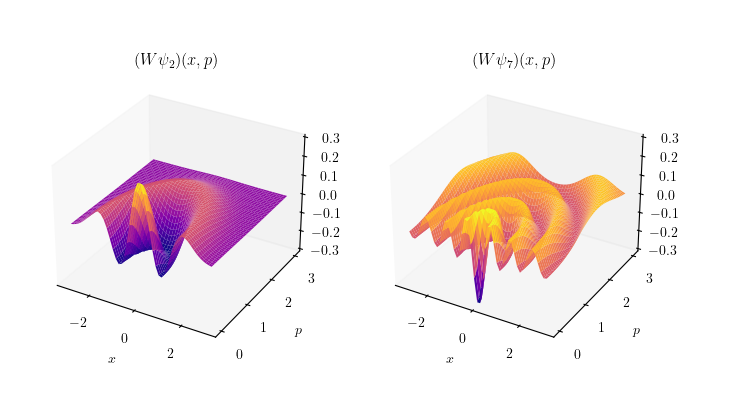
\includegraphics[width=1\textwidth]{
      imgs/harmonic_osc_wigner.png
    }
    \caption{Funciones de Wigner de los estados $\psi_3$ y
    $\psi_7$ del oscilador armónico, con $\hbar = 1$ y
    $\omega = 1$.}
    \label{fig:harmonic_osc_wigner_3_7}
  \end{figure}

  \subsection{Integrando la función de Wigner sobre rectas}

  Una caracterización de la distribución de Wigner de un
  estado cuántico es que integrando sobre ciertos conjuntos
  del espacio de fase nos brinda las probabilidades de
  observar ciertos valores de ciertos observables. Ésto es
  una generalización de las densidades de posición y de
  momentum y se ha demostrado que la función de Wigner es la
  única que tiene ésta propiedad y por lo tanto es una que
  es deseable preservar.

  No es suficiente con obtener las marginales de la posición
  y de momentum correctas para poder determinar la
  distribución conjunta, pues hay más de una. En el espacio
  de fase, podemos integrar sobre franjas formadas por
  rectas paralelas y se puede demostrar que si tenemos un
  conjunto completo de éstas ``marginales'', podemos
  recuperar la distribución conjunta sobre todo el espacio.
  [Braasch] le llama a éste conjunto de marginales un
  conjunto tomograficamente completo.

  Como se ha mencionado anteriormente, integrando sobre $x$
  ó $p$ brinda las densidades de momentum ó de posición
  respectivamente. Un resultado más general nos dice que
  podemos integrar la función de Wigner sobre una franja
  definida por dos rectas paralelas $ax + bp = c_1$ y $ax +
  bp = c_2$ en el espacio de fase y obtener la probabilidad
  de observar un valor entre $c_1$ y $c_2$ del el operador
  de Weyl
  \[
    \Op_W(ax+bp) = a \hat{x} + b \hat{p}.
  \] 
  En lugar de usar la teoría espectral para operadores
  auto-adjuntos, utilizaremos la maquinaria de Dirac.
  [2201.05911] nos dice que $a \hat{x} + b \hat{p}$ es
  esencialmente auto-adjunto y su espectro es $\R$. Entonces
  por Dirac tenemos que $\ket r$ es una eigenvector
  generalizado de $a \hat{x} + b \hat{p}$ para cada $r \in
  \sigma\left( a \hat{x} + b \hat{p} \right) = \R$. 

  UNICIDAD

  \chapter{Funciones de Wigner en el Espacio Fase Discreto}

  Resumiendo el capítulo anterior, podemos representar a un
  estado cuántico por medio de la transformación de Wigner.
  A pesar de no ser una densidad probabilística verdadera
  sobre el espacio de fase, comparte varias propiedades, en
  particular nos permite calcular los valores esperados de
  observables cuánticos y nos permite recuperar las
  densidades probabilísticas de la posición y del momentum
  integrando la función de Wigner sobre el eje de momentum o
  de posición respectivamente. Ésta última característica
  solamente es un caso partícular de una propiedad más
  general de la función de Wigner, la cual es muy útil para
  la tomografía cuántica y que de hecho la vuelva única
  entre las cuasi-distribuciones alternativas.

  Durante las últimas decadas han existido múltiples
  intentos de generalizar la función de Wigner a sistemas
  cuánticos de dimensión finita. Parte fundamental de ésta
  generalización es la definición adecuada del espacio de
  fase discreto. Para un sistema de dimensión $d$, la
  mayoría de construcciones emplean una malla de tamaño $d
  \times d$ e intentan definir una función de Wigner
  evaluada en cada par $\alpha$ de la malla. Como menciona
  Gross [THESIS], parece que existen dos caminos claros en
  la construcción de la versión discreta: un camino intenta
  definir la función de Wigner discreta de una manera
  análoga a la versión continua, i.e., identificando el
  espacio de fase discreto con las variables de posición y
  de momentum, construyendo los operadores de desplazamiento
  y luego los puntuales, para luego definir la función
  utilizando la expresión (). La ventaja de éste camino es
  que la definición discreta asemeja lo más posible al caso
  continuo y sus interpretaciones.  Ésta versión se puede
  encontrar en los trabajos de Klimov, Sanches y Soto
  [CITE], Paz [CITE], Vourdas [CITE], Gross [CITE], etc. El
  segundo camino predominante es el que intenta definir la
  función discreta a partir de la preservación de las
  propiedades más importantes del caso continuo. Ésta
  versión se debe a Gibbons y Wootters [CITE] y la idea es
  identificar una \textit{estructura cuántica} al espacio de
  fase discreto, la cual permite que la función de Wigner
  exprese las mismas propiedades que la versión discreta.
  Las ventajas de éste segundo intento, es que expone una
  relación directa con la construcción de bases mutuamente
  insesgadas y además nos ofrece una metodología que se
  puede replicar para una construcción alternativa.

  Se sabe que el número máximo de bases mutuamente
  insesgados para un sistema cuántico de dimensión $d$ es
  $d+1$, y en particular si la dimensión es una potencia de
  un número primo, entonces siempre se puede alcanzar la
  cantidad máxima [CITE]. Parece que aun es un problema
  abierto identificar la cantidad máxima para dimensiones
  que no son potencias de números primos. La construcción de
  Wootters y Gibbons requieren de la construcción explícita
  de las $d+1$ MUBs para la definición de los operadores
  puntuales y como consecuencia la definición de la función
  de Wigner. Ésto es una consecuencia natural de
  exigir que la función discreta satisfaga las mismas
  propiedades tomográficas que satisface la versión
  continua. Por éstas razones nuestro trabajo se basa en la
  metodología de Wootters, aunque hemos decidido incluir un
  resumen de la primera versión en la siguiente sección.

  \section{Construcción análoga}

  Tal como en el caso continuo, existe un mapeo del espacio
  de Hilbert al espacio de fase que se puede interpretar
  como una cuasi-distribución conjunta sobre dos variables
  `conjugadas'. Schwinger desarrolló una base ortonormal de
  $N^2$ operadores unitarios que forman una representación
  del grupo de Heisenberg-Weyl modulo su centro. Dado la
  base ortonormal de operadores, se puede describir al
  estado de un sistema utilizando los coeficientes de la
  expansión del operador de densidad en términos de la base.
  El trabajo consiste en elegir a la ``mejor'' base que
  resulte en las propiedades de la función de Wigner que
  deseamos preservar.  La idea de Wooters es construir una
  versión discreta de los operadores puntuales que preservan
  las propiedades. 

  Empezando con la transformada de Fourier discreta y
  restringiendonos a dimensiones primas impares, podremos
  trabajar en analogía al caso continuo. El grupo de
  desplazamientos de Heisenberg-Weyl nos darán los
  operadores de paridad desplazados, los cuales se usarán
  para asignar puntos del espacio de fase a operadores.

  Un sistema cuántico con una espacio de Hilbert de
  dimensión $N$ será representado por un arreglo de $N
  \times N$ puntos. Los puntos $\alpha$ estarán dados por
  los pares $(a_1,a_2)$ de elementos de un campo finito
  $\Z_n$.

  Existe una base ortonormal de $N$ elementos para nuestro
  espacio de Hilbert, correspondientes a los eigenestados de
  algún observable. Denominemos a éste observable como la
  ``posición'' y diagramaticamente denotará el eje
  horizontal. Sus eigenvalores denotarán la coordenada del
  eje horizontal. Lo que sigue es identificar las lineas
  perpendiculares al eje horizontal del espacio de fase con
  los eigenestados que corresponden a los eigenvalores. El
  eje vertical será la variable Fourier-conjugada de la
  posición llamada el ``momentum''.

  \section{Construcción de Gibbons y Wootters}

  .

  \section{Braasch}

  Para tener una versión análoga a la función de Wigner para
  el caso discreto, es necesario identificar que propiedades
  de la transformación en el caso continuo deseamos
  preservar.  Principalmente deseamos preservar (P1) el
  cálculo de los valores esperados de observables por medio
  de la integración sobre el espacio de fase, (P2) el de las
  marginales y (P3) el cálculo de probabilidades a lo largo
  de rectas en el espacio de fase.

  En la sección () se mostró que la distribución de Wigner
  satisface la siguientes propiedades:
  \begin{itemize}
    \item Realidad. Para todo $\hat{\rho}$, la distribución
      de Wigner $W(x,p)$ es real.
    \item Proyección. Para todo $\hat{\rho}$, al integrar a
      la distribuciónd e Wigner $W(x,p)$ sobre la linea $l =
      ax + bp$ en el espacio de fase nos brinda la
      probabilidad de medir $l$ del observable $a \hat{x} +
      b \hat{p}$.
    \item Hilbet-Schmidt producto interno. Para todo
      $\hat{\rho}_1$  y $\hat{\rho}_2$ se cumple que
      \[
        \Tr\left(\hat{\rho}_1 \hat{\rho}_2\right)
        = \int_{\R^{2n}} W_1(x,p) W_2(x,p) \, dx \, dp.
      \] 
    \item Traslación
  \end{itemize}

  Según [?], se puede expresar éstas propiedades en términos
  de los operadores puntuales. Los operadores puntuales
  $\Delta(x,p)$ deben ser auto-adjuntos, deben satisfacer
  las propiedades de ortogonalidad y al integrarlos sobre
  lineas en el espacio de fase nos deben de dar proyectores.

  \begin{itemize}
    \item $\hat{\Delta}(x,p)$ es auto-adjunto.
    \item ``Ortogonalidad''. 
      \[
        \Tr\left( \hat{\Delta}(x,p) \hat{\Delta}(x',p')
        \right)
        = \delta(x-x')\delta(p-p').
      \] 
    \item Supongamos que $\Pi_l$ es una proyección al
      eigenestado generalizado $a \hat{x} + b \hat{p}$ con
      eigenvalor, entonces
      \[
        \int_{\R^2} \delta(ax + bp - l) \hat{\Delta}(x,p) \,
        dx \, dp
        = \Pi_l.
      \] 
  \end{itemize}

  

  Las propiedades marginales de la función de Wigner
  continua será fundamental en la construcción de la versión
  discreta. Una propiedad marginal consiste en un conjunto
  de resultados de sumas sobre lineas paralelas. Para el
  caso discreto, una linea se define como un conjunto de
  puntos $\alpha = (a_1,a_2)$ tales que $ma_1 + na_2 = p$ 
  donde $m, n, p \in \Z_N$. Las lineas son paralelas si
  tienen los mismos valores $m,n$ y solo difieren en $p$.
  Cada linea pertenece a un conjunto de $N$ lineas paralelas
  que se llamarán ``foliación'' o ``estriación''. La
  corerspondencia entre lineas y eigenestados existe debido
  a que ambos pertenecen a conjuntos de $(N+1)$ conjuntos de
  $N$ objetos.

  Ahora debemos introducir los operadores de desplazamiento.
  Fijando un conjunto de lineas al origen, un conjunto de
  lineas no paralelas pueden ser descritas por
  desplazamientos del origen. Denotamos $\hat{D}_\alpha =
  \hat{D}(a_1,a_2)$ para un desplazamiento vertical $a_1$ y
  un desplazamiento horizontal $a_2$. Podemos generar una
  linea al elegir un desplazamiento e iterarlo. Para cada
  linea en el conjunto maximal de lineas que pasan por un
  punto, podemos generar una foliación. Por lo tanto existen
  $N(N+1)$ lineas en el espacio de fase con $N+1$ 
  foliaciones distintas.

  A la hora de vincular los observables con las lineas, la
  única restricción importante de los observables
  correspondientes a los ejes es que deben ser mutuamente
  insesgados. Ésto significa que dos conjuntos de
  eigenestados $\{\psi_m\}$ y $\{\phi_n\}$ correspondientes
  a dos observables distintos, el valor $|\langle \psi_m,
  \phi_n \rangle|^2$ debe ser independiente de $m$ y de $n$.
  En el caso discreto ésto significa que
  \[
    |\langle \psi_m, \phi_n \rangle|^2 = \frac{1}{N}.
  \] 

  \section{Anillos y campos}

  Si intentamos definir el espacio de fase discreto sobre un
  anillo como $\Z_4$ tendremos problemas a la hora de
  definir las rectas. Por ejemplo si consideramos la recta
  \[
    x + 2p = 0,
  \]
  que tiene como solución al conjunto de puntos
  \[
    \{(0,0), (2,1), (0,2), (2,3)\}.
  \] 
  Ahora, la recta 
  \[
    x = 0,
  \] 
  tiene como solución al conjunto
  \[
    \{(0,0), (0,1), (0,2), (0,3)\}.
  \] 
  Notemos que los dos conjuntos tiene una intersección con
  más de un elemento, algo que contradice nuestra noción
  geoemétrica de una linea en el espacio.

  Sea $\F_N$ un campo de $N$ elementos donde $N = r^{k}$ es
  una potencia de un número primo $r$. El primo $p$ se
  conoce como la característica de $\F_N$ y se define como
  el número entero más pequeño tal que
  \[
    1 + 1 + \ldots + 1 = 0.
  \] 
  $\F_r$ es simplemente $\Z_r$ pero $\F_N$ no es $\Z_N$.
  Para construir a $\F_N$ requerimos de un polinomio $f(x)$ 
  de grado $k$ que es irreducible en $\F_r$. Si $\alpha$ es
  una raíz de $f(x)$, el campo que obtenemos al adjuntar
  $\alpha$ a $\F_r$ es
  \[
    \F_N
    = \F_r(\alpha) \cong \F_r[x] / \langle f(x) \rangle.
  \] 
  \begin{example}
    Consideremos el anillo $\Z_4$ y el polinomio $f(x) = x^2
    + x + 1$. El campo de Galois es
    \[
      \F_2[x] / (x^2 + x + 1)
      \cong \F_2(\alpha)
      = \{0, 1, \alpha, \alpha + 1\},
    \] 
    donde $\alpha^2 + \alpha + 1 = 0$. En el campo $\F_2 =
    {0,1}$ no hay soluciones al polinomio $f(x)$ y definimos
    su solución como $\alpha$. Todo elemento de
    $\F_2(\alpha)$ tiene la forma $a_1 \alpha + a_0$, donde
    $a_j \in \F_2$, por lo tanto $\{1, \alpha\}$ es una base
    de espacio vectorial de $\F_4$ sobre $\F_2$.
  \end{example}

  El mapeo $\sigma : \alpha \to \alpha^r$ donde $\alpha \in
  \F_N$ es un automorfismo lineal de $\F_N$ llamado el
  \textit{automorfismo de Frobenius} que nos da los
  conjugados de Galois. Elementos del campo primo son
  invariantes bajo $\sigma$. Definimos la operación de traza
  de un elemento $\alpha \in \F_N$ (distinta a la traza de
  un operador lineal) como:
  \[
    \tr(\alpha) 
    = \alpha + \alpha^{r} + \alpha^{r^2} + \ldots +
    \alpha^{r^{k-1}}
    = \sum_{m=0}^{k-1} \sigma^{m}(\alpha).
  \] 
  La operación $\tr$ mapea a todo elemento del campo finito
  a un elemento del campo primo $\tr : \F_N \to \F_r$. Para
  cualquier base $E = \{e_0,e_1,\ldots,e_{N-1}\}$, existe
  una única base de campo $\tilde E = \{\tilde
  e_0,\ldots,\tilde e_{N-1}\}$ tal que $\tr(\tilde e_j e_k)
  = \delta_{jk}$. La base $\tilde E$ se llama la base dual a
  $E$. Podemos utilizar la base dual para encontrar la
  expansión única en coeficientes respecto a la base $E$ 
  para cualquier elemento $x$ del campo. Para obtener el
  componente $x_s$ del elemento $x$, hacemos
  \[
    \tr(x \tilde e_s)
    = \sum_{r}^{k} x_r \tr(e_r \tilde e_s)
    = x_s.
  \] 
  Y no mas por no mas
  \[
    \chi(\alpha)
    = \omega\left( \tr(\alpha) \right),
    \quad \alpha \in \F_N,
  \] 
  \[
    \omega(k)
    = \exp\left( \frac{2\pi i k}{p} \right),
    \quad [\chi(\alpha)]^{p} = 1, 
    \quad k \in \F_p.
  \] 

  En el caso discreto no tenemos observables que son Fourier
  conjugados de manera natural, como la posición y el
  momentum en el caso continuo. Pero podemos crear una
  estructura análoga. Considerando una base ortonormal del
  espacio de Hilbert, doptamos la notación $\ket{\hat{x},
  m}$ con $m \in \Z_N$ para denotar $m$-ésimo eigenestado
  del operador de posición. Con ésto podemos definir al
  operador de Fourier como
  \begin{definition}
    El operador de Fourier está dado por
    \begin{equation}
     \hat{\Fr}
     = \frac{1}{\sqrt{N}} 
     \sum_{m,n}^{} \omega(mn) \ket{\hat{x}; m} \bra{\hat{x};
     n},
     \quad \omega(k)
     = \exp \left( \frac{2\pi i k}{N} \right).
    \end{equation}
  \end{definition}
  Ahora podemos definir los eigenestados del ``momentum'',
  los cuales son los duales de Fourier a la base
  correspondiente a la posición. Con nuestra notación
  tenemos:
  \begin{equation}
    \ket{\hat{p}; m}
    =\hat{\Fr} \ket{\hat{x}; m}
    = \frac{1}{\sqrt{N}} \sum_{n}^{} \omega(mn)
    \ket{\hat{x};n}.
  \end{equation}
  En términos de la base de la posición, podemos expresar a
  los eigenestados de posición y de momentum como:
  \begin{equation}
    \ket{\hat{x};n}
    = \begin{bmatrix}
      0 \\
      \vdots \\
      1 \\
      \vdots \\
      0
    \end{bmatrix},
    \ket{\hat{p};m}
    = \begin{bmatrix}
      1 \\
      \omega(n) \\
      \vdots \\
      \omega\left( n(N-1) \right) 
    \end{bmatrix}.
  \end{equation}

  Es fácil probar que la aplicación repetida del operador de
  Fourier nos brinda
  \[
    \ket{\hat{x};m}
    \rightarrow{\hat{\Fr}}
    \ket{\hat{p};m}
    \rightarrow{\hat{\Fr}}
    \ket{\hat{x};-m}
    \rightarrow{\hat{\Fr}}
    \ket{\hat{p};-m}
    \rightarrow{\hat{\Fr}}
    \ket{\hat{x};m},
  \] 
  lo que prueba que $\hat{\Fr}^{4} = \id_{\H}$. Con ésto
  definimos a los operadores de posición y de momentum como
  \begin{equation}
    \hat{q}
    = \sum_{n=0}^{N-1} n \ket{\hat{x};n} \bra{\hat{x};n},
    \quad
    \hat{p}
    = \sum_{n=0}^{N-1} n \ket{\hat{p};n} \bra{\hat{p};n}.
  \end{equation}

  Los operadores $\hat{X}$ y $\hat{Z}$ de Pauli tienen la
  siguiente acción sobre los eigenestados de la posición y
  del momentum:

  \[
    \hat{Z}^{m}\ket{\hat{p};l}
    = \ket{\hat{p};l+m},
    \quad
    \hat{Z}^{m}\ket{\hat{x};l}
    = \omega(lm) \ket{\hat{x};l},
  \] 
  \[
    \hat{X}^{n}\ket{\hat{p};l}
    = \omega(-l n)\ket{\hat{p};l},
    \quad
    \hat{X}^{n}\ket{\hat{x};l}
    = \ket{\hat{x};l+n},
  \] 
  donde $l,m,n \in \Z_N$. Con ésto podemos defnir a los
  operadores de desplazamiento análogos a los del caso
  continuo:
  \begin{equation}
    \hat{D}_{\alpha}
    := \hat{D}(a_1,a_2)
    = \omega(-2^{-1} a_1 a_2) \hat{Z}^{a_1} \hat{X}^{a_2}.
  \end{equation}

  Una característica interesante es que son de traza nula
  excepto en el caso trivial:
  \[
    \Tr\left( \hat{D}(a_1,a_2) \right) 
    = \omega^{\frac{1}{2}a_1a_2} \sum_{j=0}^{N-1}
    \omega^{ja_2} \braket{j|j+a_1}
    = N \delta_{a_1,0} \delta_{a_2,0}.
  \] 
  Resulta que los operadores forman una base ortonormal
  (completa) de $N^2$ elementos respecto a la producto
  interno de Hilbert-Schmidt:
  \[
    \Tr\left( \hat{D}_\alpha^{*} \hat{D}_\beta \right) 
    = N \delta_{\alpha,\beta}.
  \] 
  Con una base a la mano, podemos descomponer a cualquier
  operador sobre $\H$ de manera única como
  \[
    \hat{A}
    = \sum_{a_1=0}^{N-1} \sum_{a_2=0}^{N-1} A_{a_1,a_2}
    \hat{D}_{a_1,a_2},
  \] 
  con los coeficientes
  \[
    A_{a_1,a_2}
    = \frac{1}{N} \Tr\left( \hat{D}_{a_1,a_2}^{*} \hat{A}
    \right)
    = \frac{1}{N} \Tr\left( \hat{D}_{-a_1,-a_2} \hat{A}
    \right).
  \] 

  Para construir un espacio de fase discreto satisfactorio
  equipado con una estructura simpléctica, requerimos
  nuestra base de $N^2$ operadores puntuales sea
  transformada por el grupo de automorfismos de los
  operadores de desplazamiento.

  \subsection{Operadores puntuales}

  Ahora buscamos construir la forma discreta de los
  operadores de paridad desplazados los cuales de nuevo se
  llamaran ocasionalmente los operadores puntuales. El
  operador de paridad (en el origen) se define como el
  cuadrado de la transformada de Fourier discreta
  \[
    \hat{\Pi}
    = \hat{\Pi}(0,0)
    = \hat{\Fr}^2.
  \] 
  En completa analogía con la versión continua, para el
  punto $\alpha$, definimos al operador puntual como
  \begin{equation}
    \hat{\Delta}(\alpha)
    = \hat{D}_\alpha \hat{\Pi} \hat{D}_{\alpha}^{-1}.
  \end{equation}
  Notemos que los operadores puntuales siguen siendo un
  involución $\hat{\Delta}(\alpha)^2 = \hat{\Pi}^2 =
  \id_{\H}$, y son unitarios. Los eigenvalores de los
  operadores puntuales son $\pm 1$ así que también son
  auto-adjuntos (?). De manera importante, tenemos las
  propiedades marginales de los operadores puntuales que
  resultan de la suma sobre lineas en el espacio de fase
  discreto. De nuevo las marginales más sencillas son las
  correspondientes al eje horizontal y el vertial (posición
  y momentum) para el operador de desplazamiento y de
  paridad. Consideremos
  \[
    \ket{\hat{x}; j}\bra{\hat{x}; j},
    \quad
    \ket{\hat{p}; j}\bra{\hat{p}; j}.
  \] 
  Para los operadores de desplazamiento tenemos
  \[
    \frac{1}{N} \sum_{a_2 = 0}^{N-1} \hat{D}(a_1,a_2)
    = \ket{\hat{p}; 2^{-1}a_1} \bra{\hat{p}; 2^{-1}a_1}
    \hat{\Delta(0,0)},
  \] 
  \[
    \frac{1}{N} \sum_{a_1=0}^{N-1} \hat{D}(a_1,a_2)
    = \ket{\hat{x}; a_2} \bra{\hat{x}; a_2}
    \hat{\Delta(0,0)},
  \] 
  \[
    \frac{1}{N} \sum_{a_1,a_2}^{} \hat{D}(a_1,a_2)
    = \hat{\Delta}(0,0).
  \]
  Para probar las primeras dos ecuaciones podemos tomar el
  funcional $\bra{\hat{x}; m}$ junto con el operdaro y el
  elemento $\ket{\hat{x}; n}$.

  Para los operadores puntuales tenemos
  \[
    \frac{1}{N} \sum_{a_2 = 0}^{N-1} \hat{\Delta}(a_1,a_2)
    = \ket{\hat{p}; a_1}\bra{\hat{p}; a_1},
  \] 
  \[
    \frac{1}{N} \sum_{a_1 = 0}^{N-1} \hat{\Delta}(a_1,a_2)
    = \ket{\hat{x}; a_2}\bra{\hat{x}; a_2},
  \] 
  \[
    \frac{1}{N} \sum_{a_1,a_2}^{} \hat{\Delta}(a_1,a_2) =
    \id_{\H}.
  \] 

  Los operadores puntuales y los de desplazamiento están
  vinculados de la misma manera que en el caso continuo, es
  decir, están conectados por transformadas de Fourier.
  \[
    \frac{1}{N}
    \sum_{a_1,a_2}^{} \hat{D}(a_1,a_2)\omega(a_2b_1-a_1b_2)
    = \hat{\Delta}(b_1,b_2)
    \iff
    \frac{1}{N} \sum_{\alpha}^{} \hat{D}_{\alpha}
    \omega^{\sigma(\beta,\alpha)} 
    = \hat{\Delta}_\beta.
  \] 
  La transformada de Fourier inversa nos brinda 
  \[
    \frac{1}{N} \sum_{\beta}^{} \hat{\Delta}_\beta
    \omega^{\sigma(\alpha,\beta)}
    = \hat{D}_\alpha.
  \] 

  El resto de las marginales se pueden obtener mediante
  transformaciones simplécticas a las marginales
  correspondientes a los ejes. Ésto corresponde con la
  versión discreta de la transformada de Radon. Dichas
  marginales nos proveen de la conección entre las
  mediciones de los observables y la reconstrucción de una
  distribución en el espacio de fase.

  \section{Wootters}

  .

  \chapter{Construcción no-estándar}

  \newpage
  \appendix

  \newpage
  \printbibliography

\end{document}
